% "{'classe':('PSI'),'chapitre':'chs_hs','type':('cours'),'titre':'Théorie des mécanismes', 'source':'','comp':('B2-16'),'corrige':True}"
\setchapterimage{Fond_CIN.png}
\setchapterpreamble[u]{\margintoc}

\chapter{Théorie des mécanismes}

\marginnote[2cm]{
\UPSTIcompetence[2]{B2-16}
}


%\marginnote[]{}

\begin{marginfigure}[4cm]
\centering
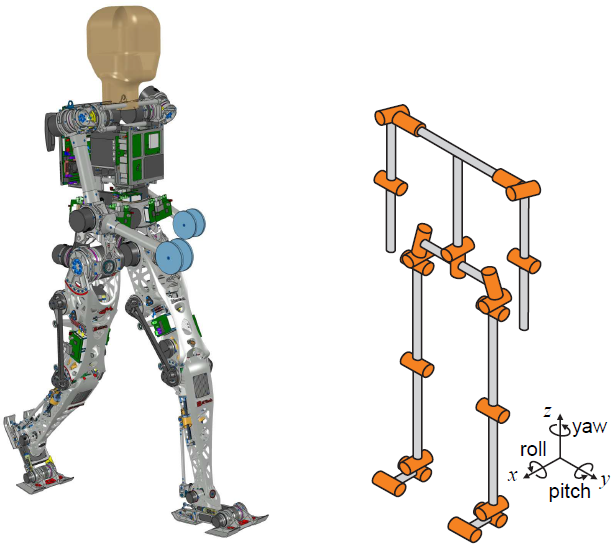
\includegraphics[width=0.6\textwidth]{lola}
\caption{Robot humanoïde Lola}
\end{marginfigure}

\begin{marginfigure}[8cm]
\centering
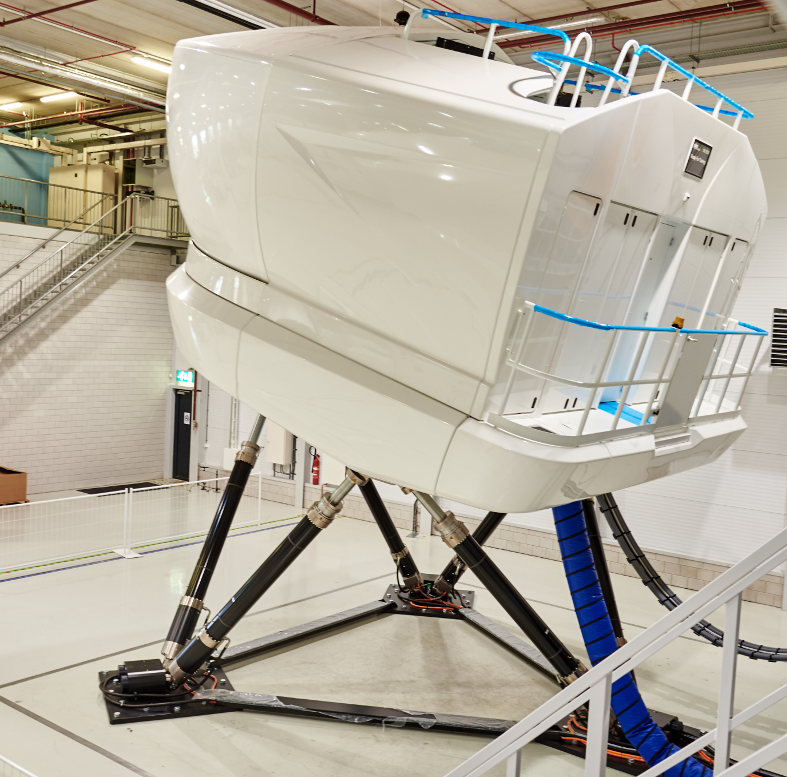
\includegraphics[width=0.5\textwidth]{simu}
\caption{Simulateur de vol Lockheed Martin}
\end{marginfigure}

\section{Degrés de mobilité}
%-----------------------------------------------------------

	
\begin{defi}[Mobilité cinématique]
On appelle $m_c=m_u+m_i$ le \textbf{degrés de mobilité cinématique} d'une liaison ou d'un mécanisme, avec :
\begin{itemize}
\item $m_u$ : le nombre de mobilités dites \textbf{utile};
\item $m_i$ : le nombre de mobilités dites \textbf{interne}.
\end{itemize}
\end{defi}

Pour une liaison seule :
\begin{itemize}
\item $m_c=0$ : liaison complète ou rigide;
\item $m_c>0$ : liaison mobile à $m_c$ degrés de liberté.
\end{itemize}

\begin{remarque}
\begin{itemize}
\item Dans un mécanisme, une mobilité utile est une mobilité \textbf{recherchée dans la fonction du mécanisme}.
On différenciera \textbf{seulement} les mobilités utiles \textbf{indépendantes}.
Si une relation existe, par exemple, entre un mouvement d'entrée et un mouvement de sortie, alors cela sera considéré comme une seule mobilité.
\item Les mobilités internes sont des mobilités indépendantes résiduelles à l'intérieur du mécanisme.
\end{itemize}
\end{remarque}


Les mobilités utiles et internes peuvent être déterminées intuitivement. Cependant, il est possible de déterminer le nombre de mobilités analytiquement. 


\begin{multicols}{2}
\begin{methode}[Méthode cinématique]

Il faut commencer par écrire la (ou les) fermetures de chaînes cinématiques. Une fermeture de chaîne permet d'écrire un système de 6 équations. On note $r_c$ le rang du système d'équations cinématiques.

On a alors $m_c = I_c -r_c$.   
\end{methode}

\begin{methode}[Méthode statique]

Il faut commencer par appliquer le PFS à chacune des pièces du système. Un PFS permet d'écrire un système de 6 équations. On note $r_S$ le rang du système d'équations statiques.

On a alors $m_c =E_S - r_s$.   
\end{methode}
\end{multicols}
		
\section{Hyperstatisme}
\subsection{Définition}
On appelle $h$ le degré d'hyperstatisme d'un mécanisme.
Il traduit l'impossibilité à résoudre un problème de mécanique, par la redondance abusive des liaisons.
			
\begin{marginfigure}
\centering

\includegraphics[width=2cm]{mickey}
\caption{Mickey, $h=M-I_c+E_y$}
\end{marginfigure}


\begin{marginfigure}
\centering

\includegraphics[width=3cm]{messi}
\caption{Messi, $h=M-E_s+I_s$}
\end{marginfigure}

\begin{multicols}{2}
\begin{methode}[en cinématique]
%On peut définir le degré d'hyperstatisme par :
$$
h=m_c-I_c+E_c
$$
\end{methode}
\begin{methode}[en statique]

$$
h=m_c-E_s+I_s
$$
\end{methode}
\end{multicols}

\begin{itemize}
\item $h=0$ : liaison ou mécanisme \textbf{isostatique};
\item $h>0$ : liaison ou mécanisme \textbf{hyperstatique};
\item si $h<0$ refaites vos calculs, \textbf{ce n'est possible} !  
\end{itemize}







\begin{defi}[Notations]

$I_c$ et $I_s$ sont respectivement les \textbf{nombres d'inconnues cinématiques et statiques} d'un système et ils dépendent du type de modélisation (2D ou 3D).


\begin{multicols}{2}
\begin{center}
\textbf{Méthode cinématique}
\end{center}

%\vspace{-.3cm}

On rappelle que le \textbf{nombre cyclomatique}  $\gamma$
est tel que $\gamma=L-S+1$ ($S$ nombre de classes d'équivalence et $L$ le nombre de liaisons).

On note $E_c$ le nombre d'équations cinématique :%et $E_{cp}$ représente le nombre d'équations complémentaires (par exemple relation dans une liaison hélicoïdale) :
\begin{itemize}
 \item en 3D : $E_c=6\gamma$;%+E_{cp}$;
 \item en 2D : $E_c=3\gamma$.%+E_{cp}$.
\end{itemize}

\vfill\null
\columnbreak

\begin{center}
\textbf{Méthode statique} 
\end{center}

%\vspace{-.3cm}

$E_s$ est le nombre d'équations statique :
\begin{itemize}
\item en 3D : $E_s=6 (S-1)$;
\item en 2D : $E_s=3 (S-1)$.
\end{itemize}

\end{multicols}
\end{defi}


\begin{remarque}[s]

\begin{itemize}
\item Un système en \textbf{chaîne ouverte} est toujours \textbf{isostatique}.%aura toujours sa mobilité générale égale à la mobilité cinématique, ainsi il sera toujours \textbf{isostatique}.
\item \textbf{Une liaison hélicoïdale a 5 inconnues statiques et 1 inconnue cinématique.}
\item Le degré d'hyperstatisme d'une chaîne bouclé \textbf{simple} ne peut pas excéder 6.
\end{itemize}
\end{remarque}


\subsection{Le système est hyperstatique... et alors ?}

Tout d'abord, d'un point de vue calcul mécanique, l'intérêt d'un système isostatique est qu'il est possible de calculer les efforts dans chacune des liaisons. Un système isostatique sera de plus facile à assembler car le positionnement des pièces les unes avec les autres est << unique >>. 

Pour les systèmes hyperstatiques, il n'est pas possible de connaître chacun des efforts. En revanche, la détermination des lois de mouvement des systèmes reste possible. Les systèmes hyperstatiques sont plus rigides que des systèmes isostatiques mais nécessitent de prendre des précautions au montage ou à la fabrication des pièces : 
\begin{itemize}
 \item les dimensions des pièces fabriquées doivent être maîtrisées;
 \item le parallélisme dans l'espace entre des axes doit être maîtrisé;
 \item du jeu doit être prévu pour garantir l'assemblage;
 \item des dispositifs de réglage peuvent être proposés.
\end{itemize}

Un système hyperstatique peut donc être plus cher à réaliser, mais peut être plus rigide et d'une plus grande durée de vie. 

Pour calculer les efforts dans un système hyperstatique, plusieurs solutions sont possibles : on peut par exemple faire des hypothèses sur une répartition d'efforts. 


\begin{methode}[Conditions de montage]
Pour déterminer les conditions de montage, il est possible d'exploiter les équations $0=0$ issues des fermetures de chaînes cinématiques.  En effet, ce nombre d'équations correspond  au degré d'hyperstatisme :
\begin{itemize}
\item une équation de type $0=0$ issue de la fermeture des vecteurs taux de rotation impose de spécifier un parallélisme;
\item une équation de type $0=0$ issue de la fermeture des vecteurs vitesse impose de spécifier une distance.
\end{itemize}
\end{methode}

Il est parfois demandé de diminuer le degré d'hyperstatisme d'un système. Pour cela, il faut rajouter des degrés de liberté à certaines liaisons, sans pour autant modifier le comportement du système.


%
%\section{Comparaison des mécanismes iso et hyperstatique}
%
%\begin{tabular}{|p{2.5cm}|p{6cm}|p{6cm}|}
%\hline \begin{center}\textbf{Mécanisme}\end{center} & \begin{center}\textbf{Avantages}\end{center} & \begin{center}\textbf{Inconvénients}\end{center} \\ 
%\hline Isostatique & Constitué de pièces plus faciles à réaliser du point de vue des contraintes dimensionnelles et géométriques.
%
%Se prête beaucoup mieux aux calculs de mécanique car on a l'assurance que les surfaces de liaison sont bien en contact.
%
% &  Souvent moins rigide qu'un mécanisme hyperstatique.
%  
%Généralement constitué d'un nombre de pièces plus important que le mécanisme hyperstatique équivalent.
%\\ 
%\hline Hyperstatique & Plus rigide qu'un système isostatique;
%
% comprend moins de pièces qu'un système isostatique pour une même fonction.
% & Constitué de pièces plus difficiles à réaliser à cause de contraintes géométriques et dimensionnelles plus importantes.
%
%Calculs mécaniques sont souvent complexes, car il faut faire intervenir la déformation des pièces.
%\\ 
%\hline 
%\end{tabular} 
%
%\section{Méthodes pour traiter un problème hyperstatique}
%
%On peut régler les problèmes de montage d'un mécanisme hyperstatique : 
%
%\begin{itemize}
%\item En donnant des jeux suffisants dans les liaisons quand cela est possible.
%\item En prévoyant des dispositifs de réglage.
%\item En jouant sur la déformation des pièces. 
%\end{itemize}

